% vim:ft=tex
% rubber: module xelatex
\subsection{Rectification}
\label{sec:rectification}

We have implemented image rectification based on our previous work in camera calibration.
We use the intrinsic and extrinsic parameters calculated by the calibration to
construct the specific perspective transformation that is required to rectify a pair of stereo images.

We obtain the following values from the calibration:
\begin{itemize}
\item $T_l, T_r$, translation vectors from the calibration object to the left
  and right camera origins respectively, in the camera reference frames.
\item $R_l, R_r$, rotation matrices from the calibration object reference system to
  the left and right camera reference systems respectively.
\item $f_l, f_r$, the focal lengths of the left and right cameras.
\end{itemize}

These parameters allow us to compute the following values:
\begin{itemize}
\item $R=R_lR_r^{-1}$, the rotation matrix from the right to the left reference
  frame.
\item $T=RT_r$-$T_l$, the translation vector from the left to the right camera
  origin, in the left camera reference frame.
\item $R_{rect}$, the rectification rotation matrix. This is computed by
  creating an orthonormal base where $X$ is the translation vector $T$, $Y$ is the cross
  product of the unit vector with $X$ (in the $Z$-axis direction), and $Z$ is the
  cross product of $X$ and $Y$.\footnote{ All vectors are normalised to unit length.}
\item $f$, the mean of the left and right focal lengths.
\end{itemize}

The rectification process then proceeds as follows. Using these values, the left image is
rectified by $R_{rect}$, and the right image is rectified by $RR_{rect}$. The
rectification coordinates are computed in 3D space, by casting the pixel
coordinates into three-dimensional coordinates, offset so that (0,0) is the
middle of the image. The $z$ component of these coordinates is the focal length. The rectification matrices are then applied to these new coordinates to get the rectified pixel coordinates.

The values are multiplied by $\frac{f}{z}$, returning the $z$ values of the new coordinates to the focal length. We use OpenCV \texttt{remap()} function to perform the actual remapping of pixels and to
interpolate non-existent pixels. Bicubic interpolation in a $4\times4$ pixel neighbourhood
is used for this last step. An example of the input and output for images acquired from a stereo camera can be seen in figure~\ref{fig:ex-rectification}.

\begin{figure}[h]
 \centering
 \subfloat[Left image (raw)] { \label{fig:sm-1} 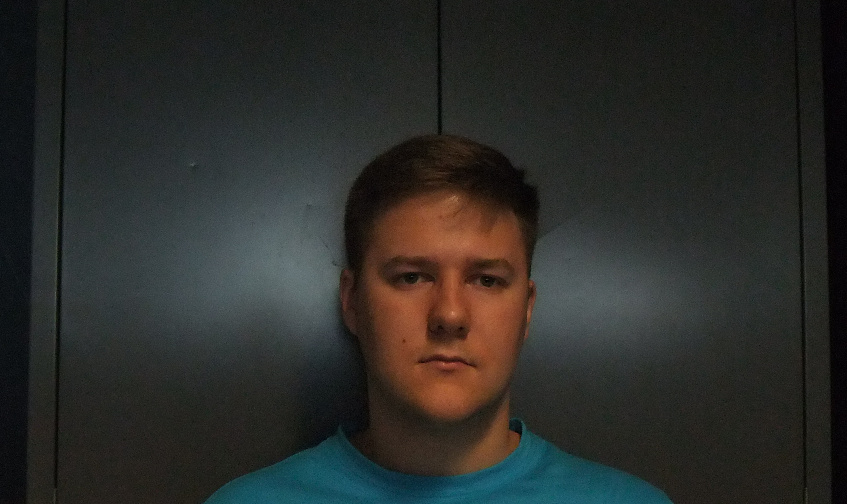
\includegraphics[trim = -2mm -2mm -2mm -2mm, width=0.4\textwidth]{example/DSCF4089_l} }
 \subfloat[Left image (rectified)] { \label{fig:sm-2} 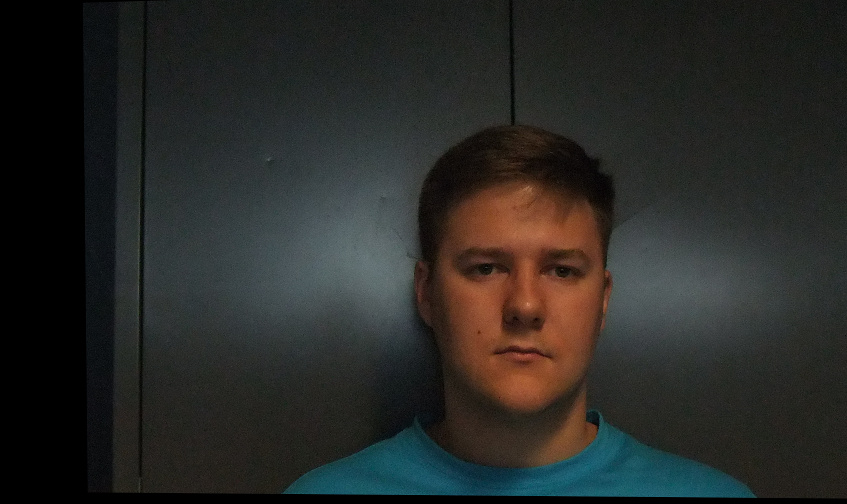
\includegraphics[trim = -2mm -2mm -2mm -2mm, width=0.4\textwidth]{example/DSCF4089rec_l} }\\
 \subfloat[Right image (raw)] { \label{fig:sm-3} 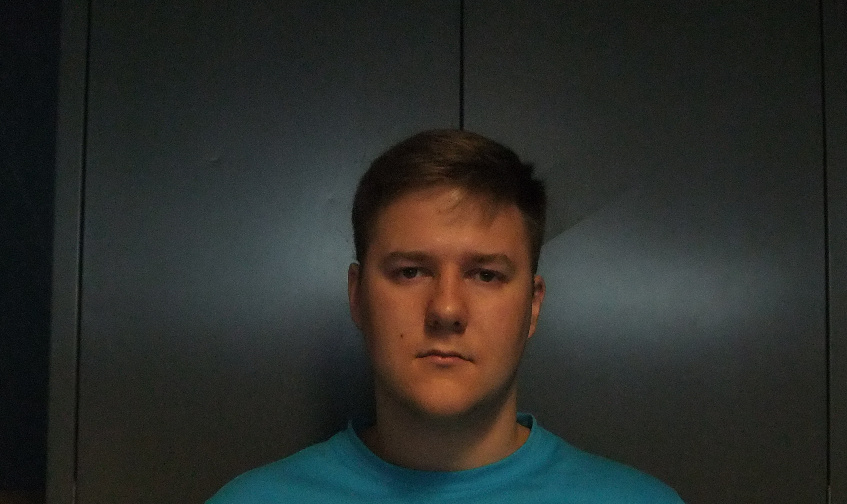
\includegraphics[trim = -2mm -2mm -2mm -2mm, width=0.4\textwidth]{example/DSCF4089_r} }
 \subfloat[Right image (rectified)] { \label{fig:sm-4} 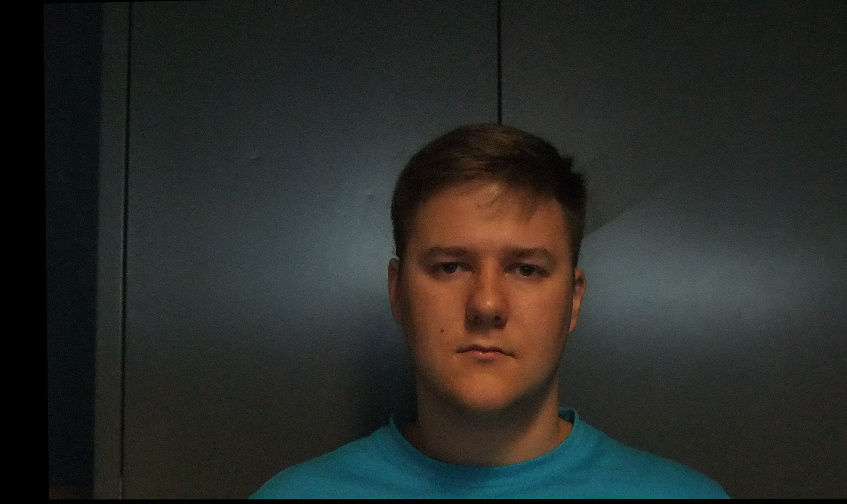
\includegraphics[trim = -2mm -2mm -2mm -2mm, width=0.4\textwidth]{example/DSCF4089rec_r} }\\
 \caption[Example of image rectification]{Example of image rectification for one stereo pair in our database. The images come from a W3 camera.}
 \label{fig:ex-rectification}
\end{figure}

\subsubsection{Testing rectification accuracy}
To test the accuracy of the rectification, we took six images with a chessboard pattern on them and rectified them. We used the OpenCV algorithm for extracting grid corners of a chessboard on the rectified images, acquiring a list of pixel positions for the corners in the image.

We then compared the $y$ coordinates of these pixels. In an accurate rectification, all the chessboard corners on a line would appear in the same scanline in the rectified image, and therefore should have the same $y$ coordinates. The disparities between $y$ coordinates can therefore be used as a measure of rectification error.

The mean errors for the six images we tested are listed in
table~\ref{tab:rectification-error}. Each image has 80 interior chessboard corners, and the image mean values are across all these corners. The overall
mean and standard deviation are also given, as the mean for all six images (i.e.
480 corners). The accuracy of the results show that overall, there is room for improvement, but they are not completely unreasonable. Our initial experiments showed that
the quality of the calibration data has a very large impact on the accuracy of the
rectification; the errors given here are for the best calibration data we were
able to obtain from the test images. A more accurate calibration could improve our rectification results considerably.

\begin{table}[h]
  \centering
  \begin{tabular}{c c c}
    \toprule
    Image & Mean error & Std dev \\
    \midrule
    DSCF4060 & 3.57  & 1.70 \\
    DSCF4061 & 3.68  & 1.60 \\
    DSCF4062 & 7.01  & 1.67 \\
    DSCF4063 & 4.40  & 1.81 \\
    DSCF4065 & 7.75  & 1.41 \\
    DSCF4066 & 7.16  & 1.84 \\
    \midrule
    Average  & 5.60  & 1.67 \\
    \bottomrule
  \end{tabular}
  \caption[Rectification errors]{Rectification errors. This table gives the mean error and
    standard deviation for the vertical displacement between the same points
    between the left and right images. These points are 80 grid corners extracted from chessboard images.}
  \label{tab:rectification-error}
\end{table}


